% Options for packages loaded elsewhere
\PassOptionsToPackage{unicode}{hyperref}
\PassOptionsToPackage{hyphens}{url}
%
\documentclass[
  a4paper,
]{article}
\usepackage{amsmath,amssymb}
\usepackage{iftex}
\ifPDFTeX
  \usepackage[T1]{fontenc}
  \usepackage[utf8]{inputenc}
  \usepackage{textcomp} % provide euro and other symbols
\else % if luatex or xetex
  \usepackage{unicode-math} % this also loads fontspec
  \defaultfontfeatures{Scale=MatchLowercase}
  \defaultfontfeatures[\rmfamily]{Ligatures=TeX,Scale=1}
\fi
\usepackage{lmodern}
\ifPDFTeX\else
  % xetex/luatex font selection
\fi
% Use upquote if available, for straight quotes in verbatim environments
\IfFileExists{upquote.sty}{\usepackage{upquote}}{}
\IfFileExists{microtype.sty}{% use microtype if available
  \usepackage[]{microtype}
  \UseMicrotypeSet[protrusion]{basicmath} % disable protrusion for tt fonts
}{}
\makeatletter
\@ifundefined{KOMAClassName}{% if non-KOMA class
  \IfFileExists{parskip.sty}{%
    \usepackage{parskip}
  }{% else
    \setlength{\parindent}{0pt}
    \setlength{\parskip}{6pt plus 2pt minus 1pt}}
}{% if KOMA class
  \KOMAoptions{parskip=half}}
\makeatother
\usepackage{xcolor}
\usepackage[margin=2.5cm]{geometry}
\usepackage{longtable,booktabs,array}
\usepackage{calc} % for calculating minipage widths
% Correct order of tables after \paragraph or \subparagraph
\usepackage{etoolbox}
\makeatletter
\patchcmd\longtable{\par}{\if@noskipsec\mbox{}\fi\par}{}{}
\makeatother
% Allow footnotes in longtable head/foot
\IfFileExists{footnotehyper.sty}{\usepackage{footnotehyper}}{\usepackage{footnote}}
\makesavenoteenv{longtable}
\ifLuaTeX
  \usepackage{luacolor}
  \usepackage[soul]{lua-ul}
\else
  \usepackage{soul}
\fi
\setlength{\emergencystretch}{3em} % prevent overfull lines
\providecommand{\tightlist}{%
  \setlength{\itemsep}{0pt}\setlength{\parskip}{0pt}}
\setcounter{secnumdepth}{3}
\ifLuaTeX
\usepackage[bidi=basic]{babel}
\else
\usepackage[bidi=default]{babel}
\fi
\babelprovide[main,import]{brazilian}
% get rid of language-specific shorthands (see #6817):
\let\LanguageShortHands\languageshorthands
\def\languageshorthands#1{}
\ifLuaTeX
  \usepackage{selnolig}  % disable illegal ligatures
\fi
\IfFileExists{bookmark.sty}{\usepackage{bookmark}}{\usepackage{hyperref}}
\IfFileExists{xurl.sty}{\usepackage{xurl}}{} % add URL line breaks if available
\urlstyle{same}
\hypersetup{
  pdflang={pt-BR},
  hidelinks,
  pdfcreator={LaTeX via pandoc}}

\renewcommand{\hl}[1]{\textcolor{red}{#1}}
\title{Priorização da manutenção arquitetural em sistemas Java Spring: análise estática, grafos semânticos e otimização multiobjetivo}
\author{Gabriel Pissinin Menossi\\Unoeste -- Universidade do Oeste Paulista\\FIPP -- Faculdade de Informática de Presidente Prudente\\DOI: ainda não possui}
\date{}

\begin{document}
\maketitle

\hypertarget{resumo}{%
\section{Resumo}\label{resumo}}

Sistemas de software acumulam erosão arquitetural ao longo tempo, e decidir por onde começar a corrigi-la costuma depender de inspeção manual e lenta. Este trabalho propõe e avalia uma abordagem automatizada que, a partir do código-fonte de sistemas Java Spring, detecta violações arquiteturais, estima o risco de cada pacote e recomenda quais pacotes refatorar primeiro, equilibrando benefício e esforço. O sistema é convertido em árvores sintáticas com o JavaParser e subsequentemente em grafos semânticos no Neo4j, sobre o qual 29 regras em Cypher detectam violações do padrão MVC e Singleton, e consultas calculam métricas de acoplamento por pacote. Um índice de risco normalizado rotula os pacotes, uma regressão logística estima a probabilidade de alto risco e o algoritmo NSGA-II busca planos de refatoração que minimizam, ao mesmo tempo, o problema restante e o esforço medido em linhas de código. A avaliação usou 978 projetos de código aberto do GitHub, com 65.139 pacotes e 120.951 violações. Os 20\% de pacotes mais graves concentraram, na mediana, 91,7\% da severidade das violações, acima do esperado por um modelo nulo proporcional ao tamanho (76,4\%; teste de Wilcoxon, p \textless{} 10⁻⁸⁰). O modelo atingiu PR-AUC de 98,1\% e recall de 97,6\% em 147 projetos de teste, mas a análise mostrou que esse desempenho reflete a reconstrução do índice estrutural: para localizar violações, o risco previsto equivaleu a ordenar os pacotes por tamanho (58,2\% da severidade nos 20\% iniciais, contra 19,9\% ao acaso). Nos projetos em que a frente de Pareto exata pôde ser enumerada, o NSGA-II alcançou 99,9\% do seu hipervolume. A contribuição é um pipeline reprodutível, evidência em larga escala da concentração de violações arquiteturais e uma análise crítica das métricas de classificação quanto a utilidade de um modelo de risco.

\textbf{Palavras-chave:} erosão arquitetural; engenharia de software baseada em busca; NSGA-II; princípio de Pareto; análise estática; refatoração.

\hypertarget{introduuxe7uxe3o}{%
\section{Introdução}\label{introduuxe7uxe3o}}

Sistemas computacionais precisam evoluir continuamente para acompanhar as demandas do mercado, e essa evolução tem custo elevado (Duvvur, 2023; Crotty \& Horrocks, 2017). Sistemas legados continuam sustentando operações críticas em empresas e governos (Irani et al., 2023), e a modernização tardia ou mal planejada desperdiça recursos (Venâncio et al., 2022). Parte importante desse custo vem da erosão arquitetural: o afastamento gradual entre a arquitetura pretendida, que torna cada nova mudança mais difícil (Perry \& Wolf, 1992; de Silva \& Balasubramaniam, 2012).

A erosão se manifesta de duas formas complementares. A primeira são as violações de regras de projeto, como uma camada de apresentação que acessa diretamente a persistência. A segunda são sintomas estruturais, como acoplamento excessivo e dependências cíclicas entre módulos (Li et al., 2022). Ambos estão associados a mais defeitos e a maior custo de manutenção (Basili et al., 1996; Zimmermann \& Nagappan, 2008; Oyetoyan et al., 2013). Detectá-los manualmente em sistemas grandes é inviável, e trabalhos recentes buscam automatizar tanto a verificação da erosão (Hu, 2023) quanto a recomendação de refatorações (Liu et al., 2024). Grafos semânticos de código são uma representação adequada para isso, porque tornam as dependências navegáveis e consultáveis (Borowski et al., 2024).

Detectar não basta: com recursos limitados, é preciso decidir por onde começar. Essa decisão envolve objetivos em conflito, como corrigir o máximo de problemas tocando o mínimo de código, e um número de alternativas que cresce exponencialmente com o número de módulos. A engenharia de software baseada em busca (SBSE) trata problemas desse tipo como otimização (Harman \& Jones, 2001; Harman, 2007), e o NSGA-II (Deb et al., 2002) é o algoritmo multiobjetivo mais usado na área (Rosa et al., 2022). Ele já foi aplicado, por exemplo, ao projeto de arquiteturas de linha de produto (Colanzi \& Vergilio, 2016; Wolschick et al., 2024) e à definição da ordem de testes de integração na presença de ciclos de dependência (Assunção et al., 2013). Uma premissa frequente nessas decisões é o princípio de Pareto: poucos módulos concentrariam a maior parte dos problemas, como já observado para defeitos de software (Fenton \& Ohlsson, 2000; Boehm \& Basili, 2001; Ostrand et al., 2005).

Há, porém, uma lacuna: poucos trabalhos combinam a detecção de regras arquiteturais específicas de um framework (como Java Spring) em larga escala, com a priorização multiobjetivo de quais módulos refatorar, e verificam empiricamente se as violações arquiteturais de fato se concentram em poucos módulos. Também é comum avaliar modelos de risco apenas por acurácia contra rótulos derivados das próprias métricas de entrada, o que pode superestimar sua utilidade.

O objetivo deste trabalho é desenvolver e avaliar uma abordagem automatizada para priorizar a manutenção arquitetural de sistemas Java Spring, combinando grafos semânticos, regras em Cypher, regressão logística e o NSGA-II.

As contribuições são: (i) um pipeline aberto e reprodutível, do código-fonte à recomendação; (ii) evidência, em 978 projetos, de que as violações se concentram em poucos pacotes além do esperado pelo tamanho; (iii) uma formulação custo × benefício do NSGA-II verificada contra a frente de Pareto exata; e (iv) uma análise crítica que mostra quando a acurácia de um modelo de risco não corresponde à sua capacidade de localizar violações.

\hypertarget{material-e-muxe9todos}{%
\section{Material e métodos}\label{material-e-muxe9todos}}

\hypertarget{desenho-da-soluuxe7uxe3o}{%
\subsection{Desenho da solução}\label{desenho-da-soluuxe7uxe3o}}

A solução é composta por três serviços (Figura 1). Um serviço em Java (Java 25, Spring Boot 4.1.1) analisa o código e constrói o grafo no Neo4j 5.26; um serviço em Python 3.12 calcula o risco e executa o NSGA-II; e uma aplicação web em Go 1.26 orquestra as etapas e apresenta os resultados.

\begin{figure}[htbp]
\centering
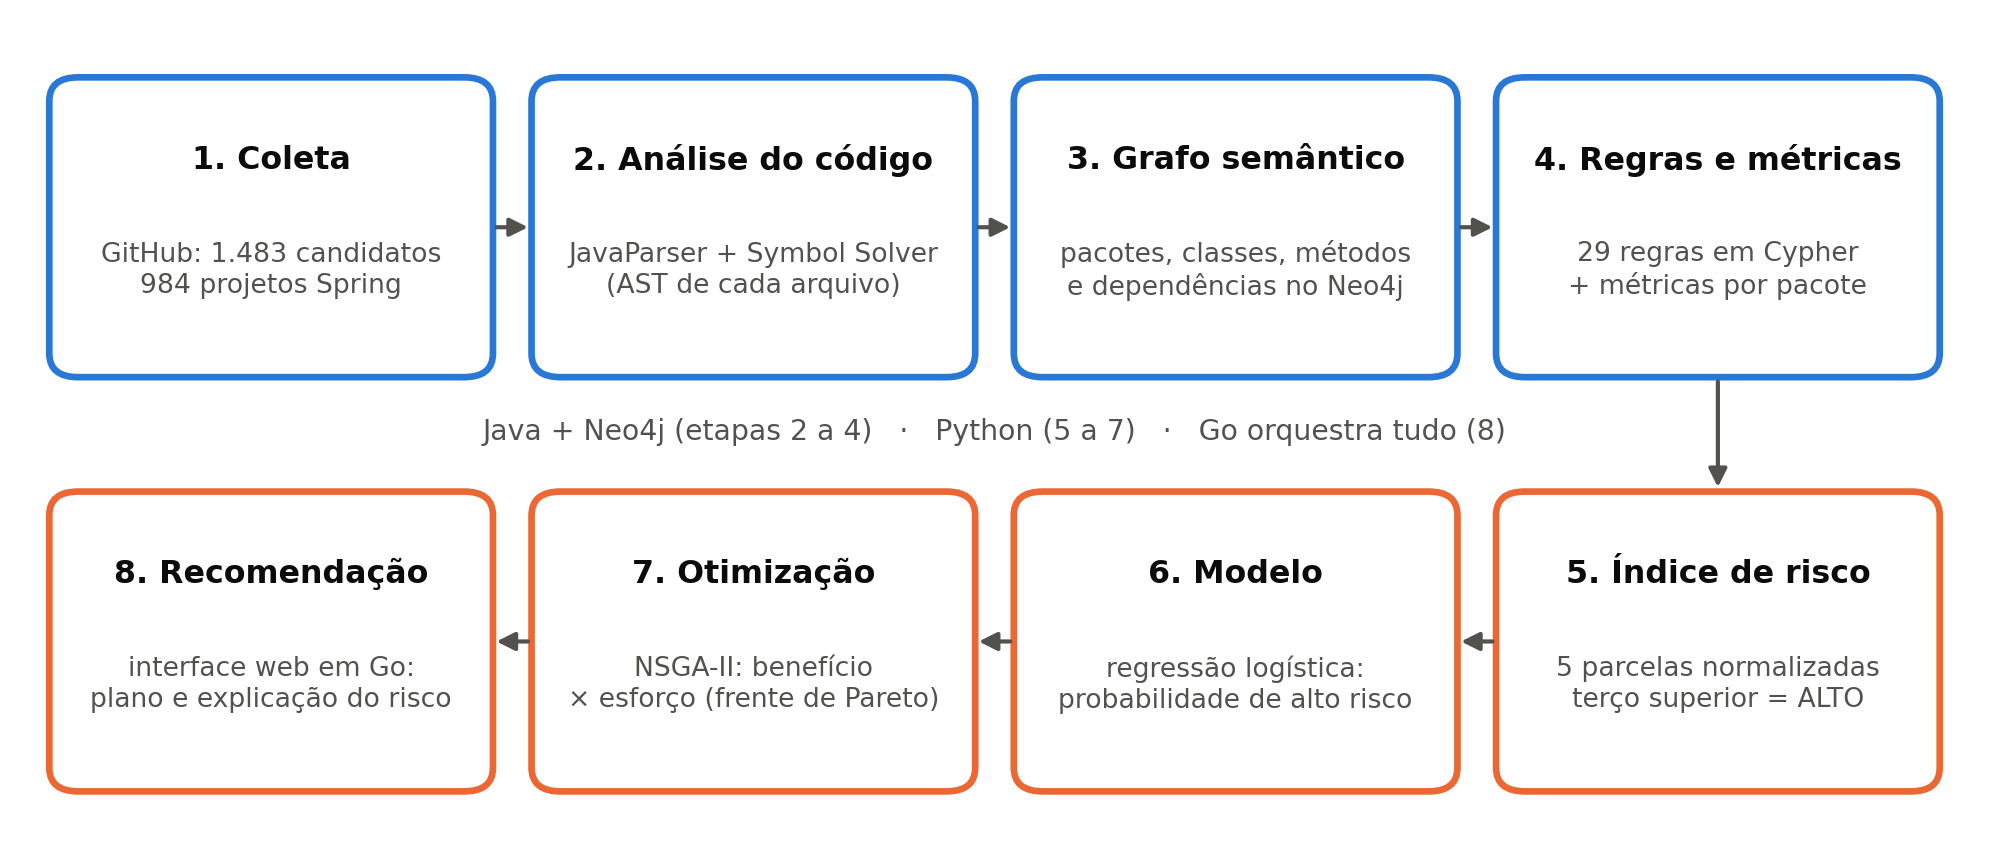
\includegraphics[width=\linewidth,height=0.82\textheight,keepaspectratio]{figures/image5.png}
\caption{Fluxo da abordagem, da coleta dos projetos à recomendação.}
\end{figure}


\hypertarget{corpus-e-crituxe9rios-de-seleuxe7uxe3o}{%
\subsection{Corpus e critérios de seleção}\label{corpus-e-crituxe9rios-de-seleuxe7uxe3o}}

Os projetos foram coletados pela API REST de busca do GitHub com os critérios: linguagem Java, ao menos 20 estrelas, tamanho mínimo de 500 KB e último \emph{push} nos 24 meses anteriores à coleta, para privilegiar projetos com manutenção ativa. Dos 1.483 candidatos, 984 foram confirmados como Spring pela presença do framework nos arquivos de build (Maven ou Gradle). Os repositórios foram clonados com profundidade 1 e analisados um a um; 979 geraram grafo e 978 tiveram métricas por pacote. A Tabela 1 resume o corpus.

\textbf{Tabela 1.} Corpus e divisão entre treino, validação e teste.

\begin{longtable}[]{@{}
  >{\raggedright\arraybackslash}p{(\columnwidth - 8\tabcolsep) * \real{0.3293}}
  >{\raggedright\arraybackslash}p{(\columnwidth - 8\tabcolsep) * \real{0.1585}}
  >{\raggedright\arraybackslash}p{(\columnwidth - 8\tabcolsep) * \real{0.1951}}
  >{\raggedright\arraybackslash}p{(\columnwidth - 8\tabcolsep) * \real{0.1463}}
  >{\raggedright\arraybackslash}p{(\columnwidth - 8\tabcolsep) * \real{0.1463}}@{}}
\toprule\noalign{}
\begin{minipage}[b]{\linewidth}\raggedright
\textbf{Medida}
\end{minipage} & \begin{minipage}[b]{\linewidth}\raggedright
\textbf{Treino}
\end{minipage} & \begin{minipage}[b]{\linewidth}\raggedright
\textbf{Validação}
\end{minipage} & \begin{minipage}[b]{\linewidth}\raggedright
\textbf{Teste}
\end{minipage} & \begin{minipage}[b]{\linewidth}\raggedright
\textbf{Total}
\end{minipage} \\
\midrule\noalign{}
\endhead
\bottomrule\noalign{}
\endlastfoot
Projetos & 685 & 146 & 147 & 978 \\
Pacotes & 47.654 & 9.112 & 8.373 & 65.139 \\
Pacotes de alto risco & 32,8\% & 33,5\% & 36,6\% & 33,4\% \\
\end{longtable}

O corpus soma 4,84 milhões de nós, 11,4 milhões de arestas e 12,9 milhões de linhas de código em métodos. A mediana é de 21 pacotes por projeto (máximo de 2.776); 31,3\% dos pacotes têm ao menos uma violação.

\hypertarget{pruxe9-processamento-do-cuxf3digo-ao-grafo}{%
\subsection{Pré-processamento: do código ao grafo}\label{pruxe9-processamento-do-cuxf3digo-ao-grafo}}

Cada arquivo .java é convertido em uma árvore sintática abstrata pelo JavaParser 3.26.3, com o Symbol Solver configurado para resolver tipos do próprio projeto, do JDK e das bibliotecas disponíveis. A análise é feita sobre o código-fonte, sem compilar o projeto, o que viabiliza processar centenas de repositórios de terceiros. O grafo tem nós de projeto, pacote, arquivo, tipo, método, campo e construtor, e arestas de contenção, declaração, dependência entre tipos, chamada de método e uso de tipos (campo, parâmetro, retorno, instanciação, herança, implementação e exceção). Ele é gravado no Neo4j em lotes de 2.000 operações, como uma forma de evitar erros devido a uma quantidade de gravação muito grande.

\hypertarget{detecuxe7uxe3o-de-violauxe7uxf5es-e-muxe9tricas}{%
\subsection{Detecção de violações e métricas}\label{detecuxe7uxe3o-de-violauxe7uxf5es-e-muxe9tricas}}

Sobre o grafo são executadas 29 regras em Cypher: 18 de Spring MVC e 11 do padrão Singleton. As regras de Spring MVC cobrem dependências indevidas entre camadas, uso de @Transactional, injeção de dependência, tratamento de exceções e Controllers com responsabilidades excessivas; três delas são heurísticas baseadas no nome dos métodos. Cada ocorrência gera um nó de violação ligado à classe responsável, com severidade HIGH, MEDIUM, LOW ou INFO.

Para cada pacote, consultas em Cypher calculam: o acoplamento aferente (fan-in, classes de outros pacotes que dependem dele); o acoplamento eferente (fan-out, soma das dependências de suas classes para classes de outros pacotes); as dependências cruzadas (número de pacotes distintos dos quais depende); as classes que participam de ciclos de dependência de até cinco classes; a instabilidade I = fan-out / (fan-in + fan-out) (Martin, 2003); e as contagens de violações por severidade. Só entram dependências entre classes do próprio projeto. O grafo é então exportado e removido do Neo4j.

\hypertarget{uxedndice-de-risco-e-ruxf3tulo}{%
\subsection{Índice de risco e rótulo}\label{uxedndice-de-risco-e-ruxf3tulo}}

A severidade ponderada de um pacote é 3*HIGH + 2*MEDIUM + 1*LOW + 0,5*INFO. O índice de risco combina cinco parcelas normalizadas entre 0 e 1 pelos valores mínimo e máximo do corpus (Equação 1):

risco = 0,2 * {[}N(severidade) + N(violações Singleton) + N(classes em ciclo) + N(dependências cruzadas) + N(fan-out){]} (1)

em que N(x) = (x − mín) / (máx − mín). Os pacotes do terço superior do índice (risco ≥ 0,00462) recebem o rótulo ALTO RISCO, usado como classe positiva no treino.

\hypertarget{modelo-de-risco}{%
\subsection{Modelo de risco}\label{modelo-de-risco}}

A regressão logística estima a probabilidade de alto risco a partir de 11 medidas estruturais: fan-in, fan-out, classes em ciclo, dependências cruzadas e sete medidas do subgrafo do pacote (nós, arestas, tipos, Controllers, Services, Repositories e grau médio). As contagens e a severidade das violações são excluídas das entradas. As entradas são padronizadas com média e desvio do treino, e o treino usa gradiente descendente em lote, 600 épocas, taxa de aprendizado 0,08, regularização L2 0,01 e pesos que equilibram as classes. A função de custo é convexa, por isso não se usou parada antecipada.

Os projetos foram divididos em 70\% para treino, 15\% para validação e 15\% para teste, \textbf{por projeto} (todos os pacotes de um projeto ficam na mesma parte), com estratificação pela classe predominante e semente 42. A validação foi usada apenas para calibrar o limiar de decisão: o maior recall com precisão de ao menos 80\%, que resultou em 0,356.

\hypertarget{otimizauxe7uxe3o-multiobjetivo}{%
\subsection{Otimização multiobjetivo}\label{otimizauxe7uxe3o-multiobjetivo}}

Cada solução do NSGA-II é um vetor binário com um gene por pacote candidato (1 = refatorar). São candidatos os pacotes com violação e os pacotes com alto risco previsto; nos pacotes que apenas agrupam subpacotes, o risco previsto é ignorado, porque suas medidas incluem as dos subpacotes. Os dois objetivos, minimizados, são o problema restante (1 − benefício) e o esforço, medido como a fração das linhas de código do projeto contidas nos pacotes escolhidos. O benefício de um plano é 0,5 * a fração da severidade das violações que ele cobre + 0,5 * a fração do risco * tamanho que ele cobre. O NSGA-II usa torneio binário por posição na frente e distância de aglomeração, cruzamento de um ponto (probabilidade 0,9), mutação bit a bit (probabilidade 1/n) e elitismo. A população e o número de gerações crescem com o número de candidatos, de 50 até 200 indivíduos e de 50 até 300 gerações. Da frente final, a ferramenta recomenda o ponto de joelho, o mais distante da reta entre os extremos da curva (Satopää et al., 2011), e o melhor plano com até 20\% de esforço.

\hypertarget{muxe9todos-de-comparauxe7uxe3o-e-muxe9tricas}{%
\subsection{Métodos de comparação e métricas}\label{muxe9todos-de-comparauxe7uxe3o-e-muxe9tricas}}

Para cada projeto com ao menos cinco pacotes e alguma violação, ordenaram-se os pacotes pela severidade e calculou-se S20, a fração da severidade nos primeiros 20\% dos pacotes (com interpolação para frações de pacote). Como controles, mediu-se a fração das linhas de código nesses pacotes e construiu-se um modelo nulo que redistribui as violações do projeto ao acaso, proporcionalmente às linhas de código de cada pacote (20 sorteios por projeto). A diferença entre S20 real e nulo foi testada com o teste de postos sinalizados de Wilcoxon (Wilcoxon, 1945). A sensibilidade foi avaliada excluindo a regra mais frequente (MVC14), as duas regras Singleton mais amplas (SG\_06 e SG\_11) ou mantendo só violações HIGH ou só de camadas.

No conjunto de teste, relatam-se acurácia, precisão, recall, F1 e PR-AUC, adequada a classes desequilibradas (Saito \& Rehmsmeier, 2015), com intervalos de confiança de 95\% por reamostragem de projetos (\emph{bootstrap}, 1.000 amostras; Efron \& Tibshirani, 1993). Duas linhas de base mostram quanto do rótulo é explicado diretamente pelas entradas: a regra "três ou mais dependências cruzadas ou alguma classe em ciclo" e a parte estrutural do índice. Para medir a utilidade do risco na localização de violações, os pacotes de cada projeto de teste foram ordenados pelo risco previsto, pelo tamanho em linhas de código, ao acaso e pela severidade real (ótimo), medindo a fração da severidade capturada pelos 20\% iniciais e o Popt (Mende \& Koschke, 2010).

O NSGA-II foi executado nos 147 projetos de teste. Com até 16 candidatos, a frente exata foi obtida por enumeração e comparada com a encontrada; acima disso, o hipervolume (Zitzler \& Thiele, 1999) foi comparado com o de um método guloso que acumula pacotes em ordem de benefício ÷ esforço, e a busca foi repetida com cinco sementes. Mediram-se também o tempo de execução, com seis projetos processados em paralelo numa máquina de oito núcleos, e a comparação com a formulação anterior, de cinco objetivos com fatores de melhoria simulados, limitada a 120 s por projeto.

\hypertarget{protocolo-e-reproduuxe7uxe3o}{%
\subsection{Protocolo e reprodução}\label{protocolo-e-reproduuxe7uxe3o}}

Os parâmetros, a divisão e as sementes são fixos. Os scripts de análise leem o corpus e aplicam o modelo treinado, sem retreiná-lo, e gravam todos os números e figuras. O código dos três serviços e dos scripts está disponível no repositório do projeto.

\hypertarget{resultados-e-discussuxe3o}{%
\section{Resultados e discussão}\label{resultados-e-discussuxe3o}}

\hypertarget{panorama-das-violauxe7uxf5es}{%
\subsection{Panorama das violações}\label{panorama-das-violauxe7uxf5es}}

A Figura 2 mostra a distribuição das 120.951 violações. Práticas do Spring dominam (70,8\%), com destaque para a injeção por campo (44,0\%) e para métodos de leitura e escrita sem @Transactional (17,8\% e 8,8\%). Violações de camada propriamente ditas, como um Controller que usa um Repository, somam 4,0\%. As regras Singleton respondem por 21,1\%, mas a análise revelou que duas delas são amplas demais: SG\_06 marca todo enum e SG\_11 marca toda classe com construtor privado. Esse é um limite das regras discutido adiante.

\begin{figure}[htbp]
\centering
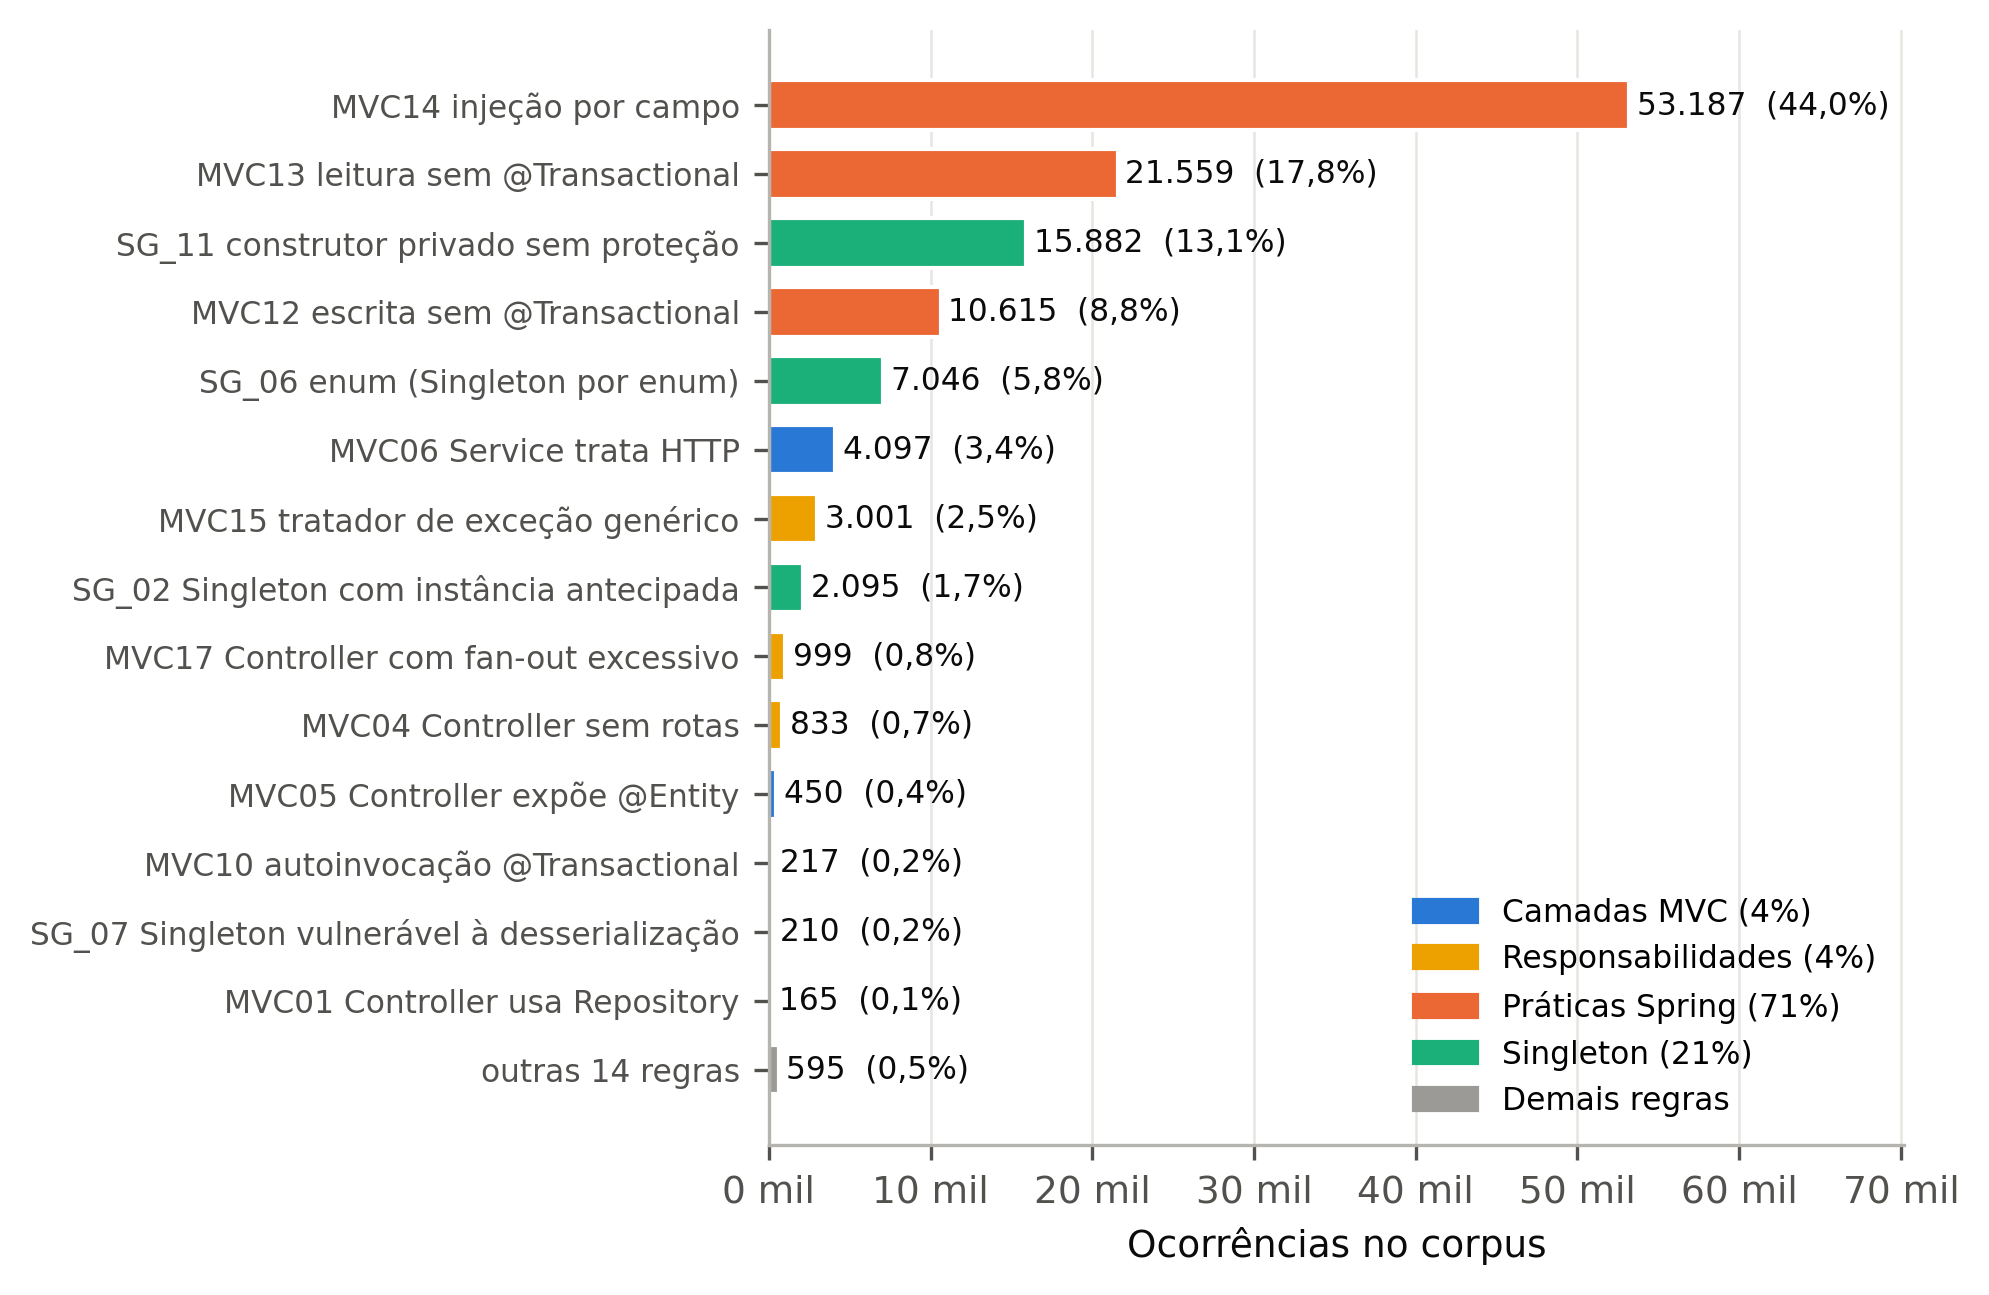
\includegraphics[width=\linewidth,height=0.82\textheight,keepaspectratio]{figures/image4.png}
\caption{Ocorrências por regra no corpus, agrupadas por categoria.}
\end{figure}


\hypertarget{concentrauxe7uxe3o-das-violauxe7uxf5es}{%
\subsection{Concentração das violações}\label{concentrauxe7uxe3o-das-violauxe7uxf5es}}

Em 891 projetos, os 20\% de pacotes mais graves concentraram, na mediana, 91,7\% da severidade (IC 95\% da mediana: 90,5\% a 92,9\%; quartis: 78,3\% e 98,6\%), e 73,8\% dos projetos passaram de 80\% (Figura 3). O tamanho explica parte disso: esses pacotes contêm 44,8\% das linhas de código, e o modelo nulo proporcional ao tamanho produziria uma concentração mediana de 76,4\%. Ainda assim, a concentração real superou a nula em 76,7\% dos projetos, com diferença mediana de 10,3 pontos percentuais (Wilcoxon, p \textless{} 10⁻⁸⁰). A conclusão se mantém, e se fortalece, nas análises de sensibilidade (Tabela 2).

\begin{figure}[htbp]
\centering
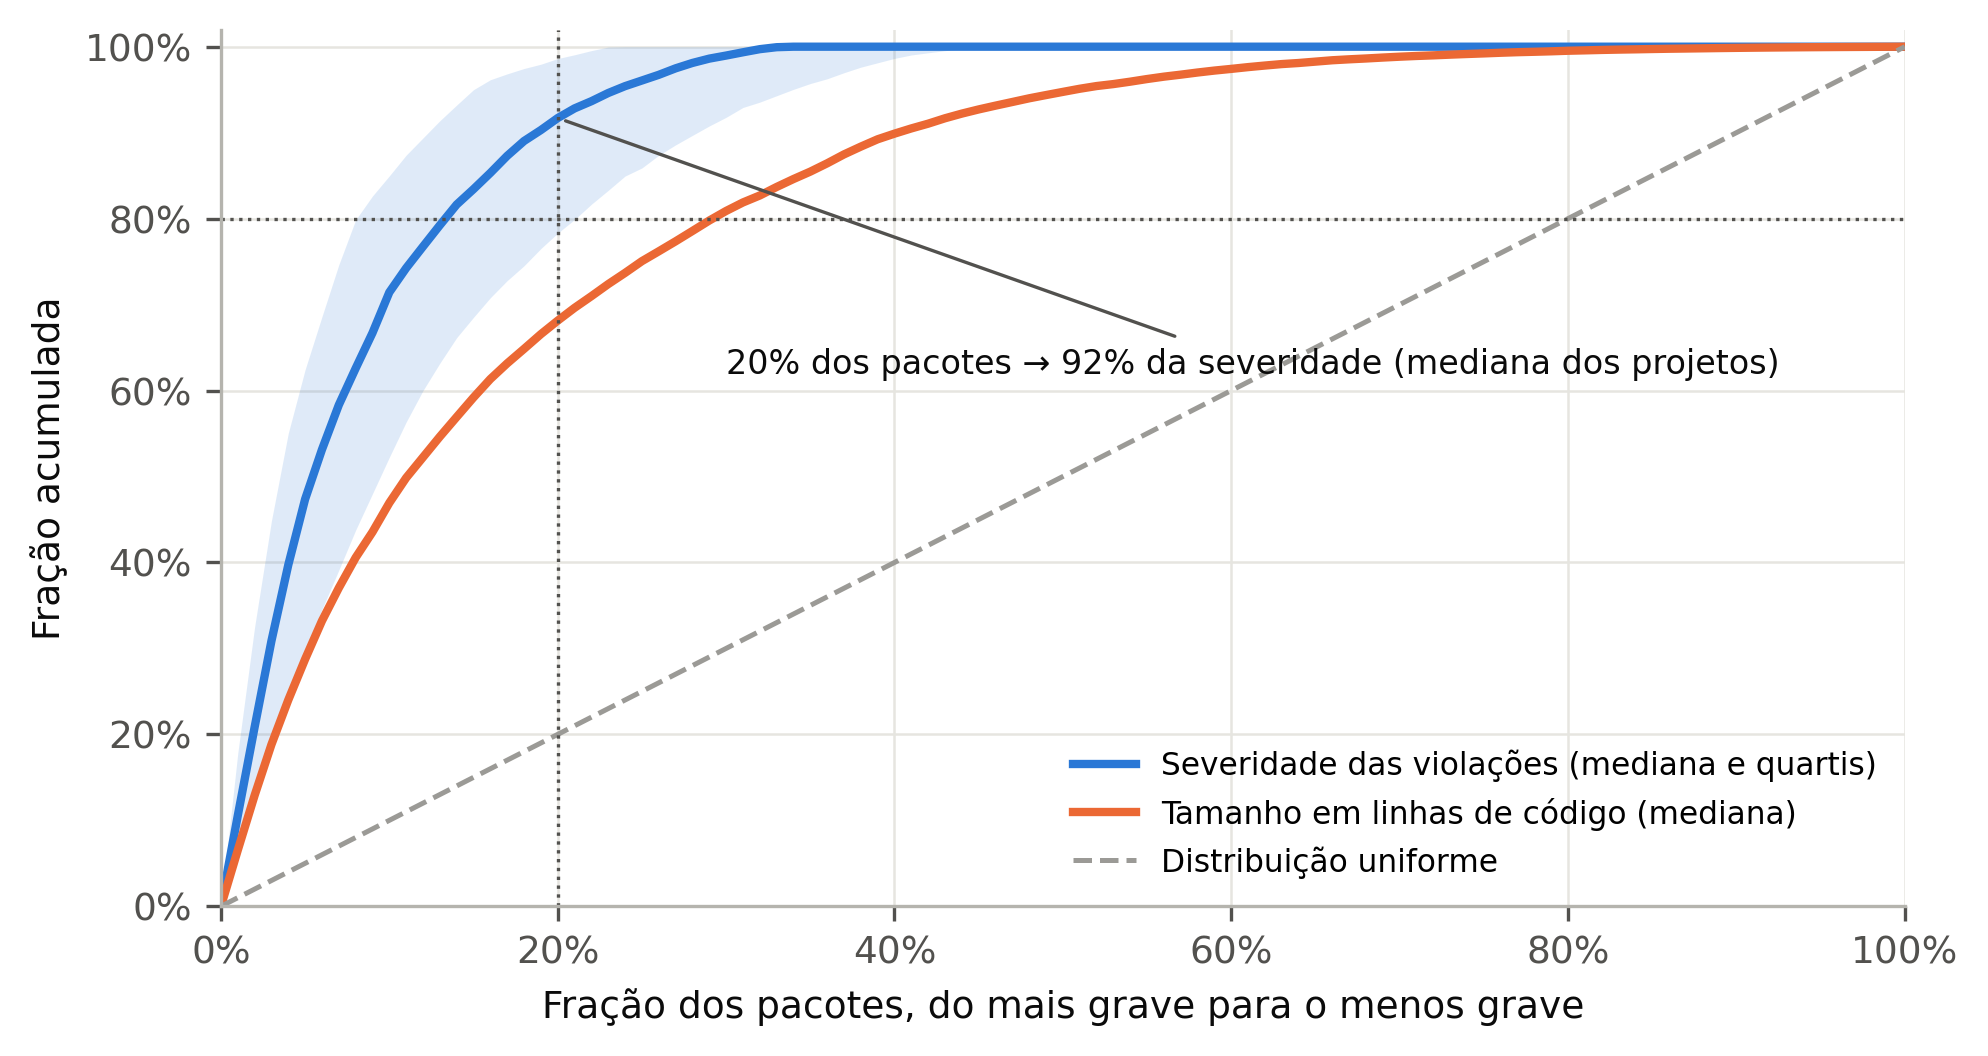
\includegraphics[width=\linewidth,height=0.82\textheight,keepaspectratio]{figures/image3.png}
\caption{Fração acumulada da severidade e das linhas de código por fração de pacotes (mediana e quartis entre projetos).}
\end{figure}


\textbf{Tabela 2.} Concentração da severidade (S20) por variante da contagem.

\begin{longtable}[]{@{}
  >{\raggedright\arraybackslash}p{(\columnwidth - 6\tabcolsep) * \real{0.3580}}
  >{\raggedright\arraybackslash}p{(\columnwidth - 6\tabcolsep) * \real{0.1852}}
  >{\raggedright\arraybackslash}p{(\columnwidth - 6\tabcolsep) * \real{0.1481}}
  >{\raggedright\arraybackslash}p{(\columnwidth - 6\tabcolsep) * \real{0.2840}}@{}}
\toprule\noalign{}
\begin{minipage}[b]{\linewidth}\raggedright
\textbf{Variante}
\end{minipage} & \begin{minipage}[b]{\linewidth}\raggedright
\textbf{Projetos}
\end{minipage} & \begin{minipage}[b]{\linewidth}\raggedright
\textbf{S20 mediano}
\end{minipage} & \begin{minipage}[b]{\linewidth}\raggedright
\textbf{Projetos com S20 ≥ 80\%}
\end{minipage} \\
\midrule\noalign{}
\endhead
\bottomrule\noalign{}
\endlastfoot
Todas as regras & 891 & 91,7\% & 73,8\% \\
Sem MVC14 (injeção por campo) & 870 & 100,0\% & 87,0\% \\
Sem SG\_06 e SG\_11 & 867 & 98,4\% & 87,1\% \\
Só severidade HIGH & 334 & 100,0\% & 99,1\% \\
Só violações de camada & 276 & 100,0\% & 98,9\% \\
\end{longtable}

O resultado replica para violações arquiteturais a concentração observada para defeitos (Fenton \& Ohlsson, 2000; Boehm \& Basili, 2001; Ostrand et al., 2005). Em termos práticos, uma equipe que inspecione um quinto dos pacotes encontra a maior parte da severidade; em termos de código, porém, isso corresponde a cerca de 45\% das linhas, o que reforça a necessidade de considerar o esforço, como faz o NSGA-II. As variantes mais restritas produzem concentrações próximas de 100\% em parte porque as violações ficam mais raras.

\hypertarget{desempenho-e-utilidade-do-modelo}{%
\subsection{Desempenho e utilidade do modelo}\label{desempenho-e-utilidade-do-modelo}}

No teste (147 projetos, 8.373 pacotes), o modelo obteve acurácia de 90,2\% (IC 95\%: 89,2\% a 91,0\%), precisão de 80,1\% (74,9\% a 83,4\%), recall de 97,6\% (96,2\% a 98,4\%), F1 de 88,0\% (84,3\% a 90,3\%) e PR-AUC de 98,1\% (96,7\% a 98,8\%) (Figura 4). Os valores de treino foram próximos (acurácia de 91,1\% e PR-AUC de 97,6\%), sem sinal de sobreajuste. Excluindo os 17 projetos de teste com estrutura de pacotes quase idêntica à de um projeto de treino (Jaccard ≥ 0,8), os resultados praticamente não mudaram (acurácia de 90,0\% e PR-AUC de 98,2\%).

\begin{figure}[htbp]
\centering
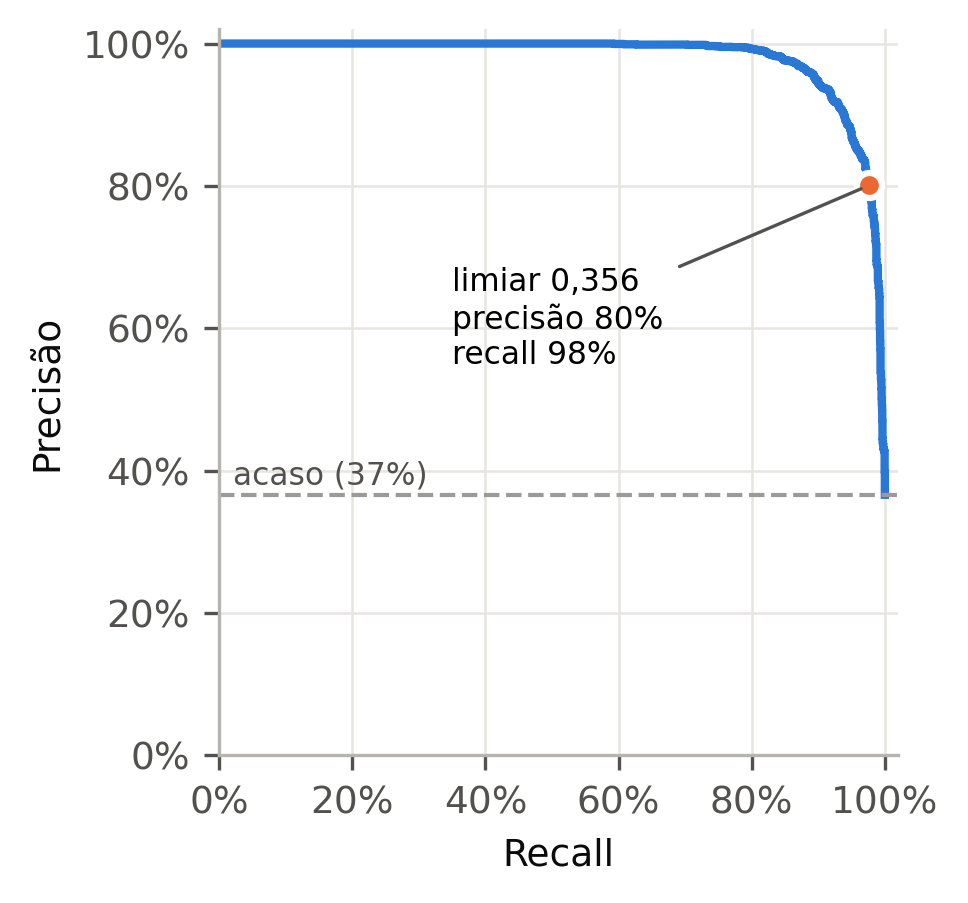
\includegraphics[width=\linewidth,height=0.82\textheight,keepaspectratio]{figures/image1.png}
\caption{Curva precisão × recall no conjunto de teste, com o ponto do limiar calibrado.}
\end{figure}

\hl{Vou tirar esse acaso, ficou confuso para entender de primeira}.

Esses números, no entanto, devem ser lidos com cautela. A regra de uma linha "três ou mais dependências cruzadas ou alguma classe em ciclo" acerta 95,4\% dos rótulos do teste, e a parte estrutural do índice acerta 96,8\%. Com os limites do corpus, três dependências cruzadas sozinhas já ultrapassam o corte de ALTO RISCO, e essa parcela responde por cerca de 78\% do índice médio dos pacotes de alto risco. Os pesos do modelo confirmam a leitura: dependências cruzadas (2,86) e fan-out (0,95) dominam, seguidos pelo grau médio (0,54) e pelas classes em ciclo (0,46). O modelo, portanto, reconstrói um índice que é, em boa parte, função das próprias entradas.

Por isso a avaliação decisiva é se o risco previsto, que não recebe as violações, as localiza (Figura 5). Nos 136 projetos de teste com violações, os 20\% de pacotes de maior risco capturaram, na mediana, 58,2\% da severidade (IC 95\%: 51,6\% a 64,8\%), bem acima do acaso (19,9\%; Wilcoxon, p \textless{} 10⁻²⁰) e abaixo do ótimo (88,6\%). Os pacotes marcados como alto risco tinham violação em 50,3\% dos casos, contra 18,5\% dos demais. Porém, ordenar os pacotes apenas pelo número de linhas de código produziu a mesma captura mediana (58,2\%; diferença não significativa, p = 0,54), Popt semelhante (0,855 contra 0,865) e PR-AUC ligeiramente maior para a presença de violação (0,58 contra 0,56). Para localizar violações, o risco previsto equivale, na prática, a olhar primeiro os pacotes maiores.

\begin{figure}[htbp]
\centering
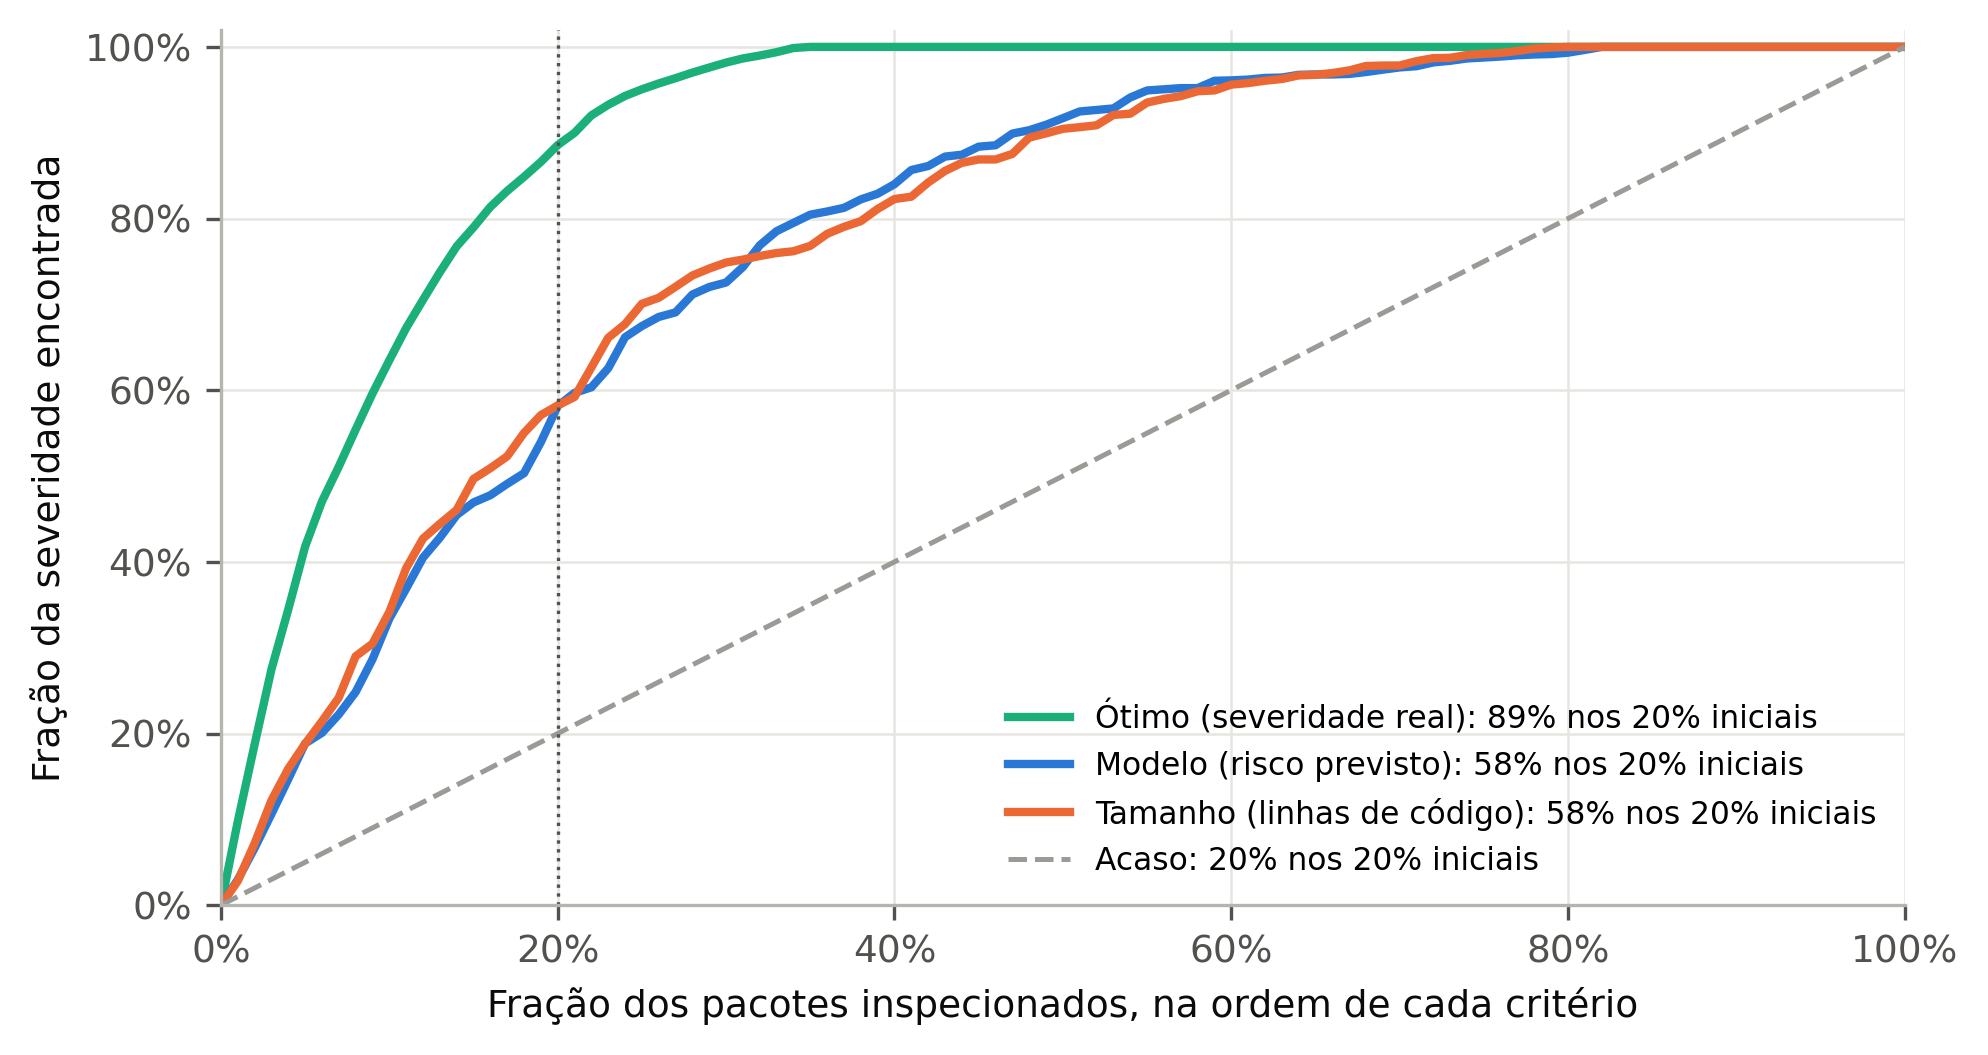
\includegraphics[width=\linewidth,height=0.82\textheight,keepaspectratio]{figures/image8.png}
\caption{Fração da severidade encontrada ao inspecionar os pacotes na ordem do risco previsto, do tamanho, ao acaso e da severidade real (mediana dos projetos de teste).}
\end{figure}

\hl{Retira a linha que mostra o acaso}.

Esse resultado não invalida a abordagem, mas delimita o papel de cada componente. A localização exata das violações é feita pelas regras; o modelo resume um risco estrutural, interpretável fator a fator, que inclui pacotes sem violação. Dos 21.739 pacotes de alto risco do corpus, 43,7\% não têm violação, e 37,6\% do total estão nessa classe por dependerem de três ou mais pacotes (Figura 6). Acoplamento excessivo e ciclos são sintomas estruturais de erosão reconhecidos na literatura (Martin, 2003; Melton \& Tempero, 2007; Li et al., 2022), não capturados pelas regras MVC e Singleton. Ao mesmo tempo, 60,2\% dos pacotes com violação são de alto risco e só 6,9\% são de baixo risco, o que mostra que as duas visões se sobrepõem. A escolha de pesos iguais no índice mostrou-se pouco sensível: em 500 sorteios de pesos aleatórios, o conjunto de alto risco manteve semelhança mediana de 0,92 (Jaccard) com o original.

\begin{figure}[htbp]
\centering
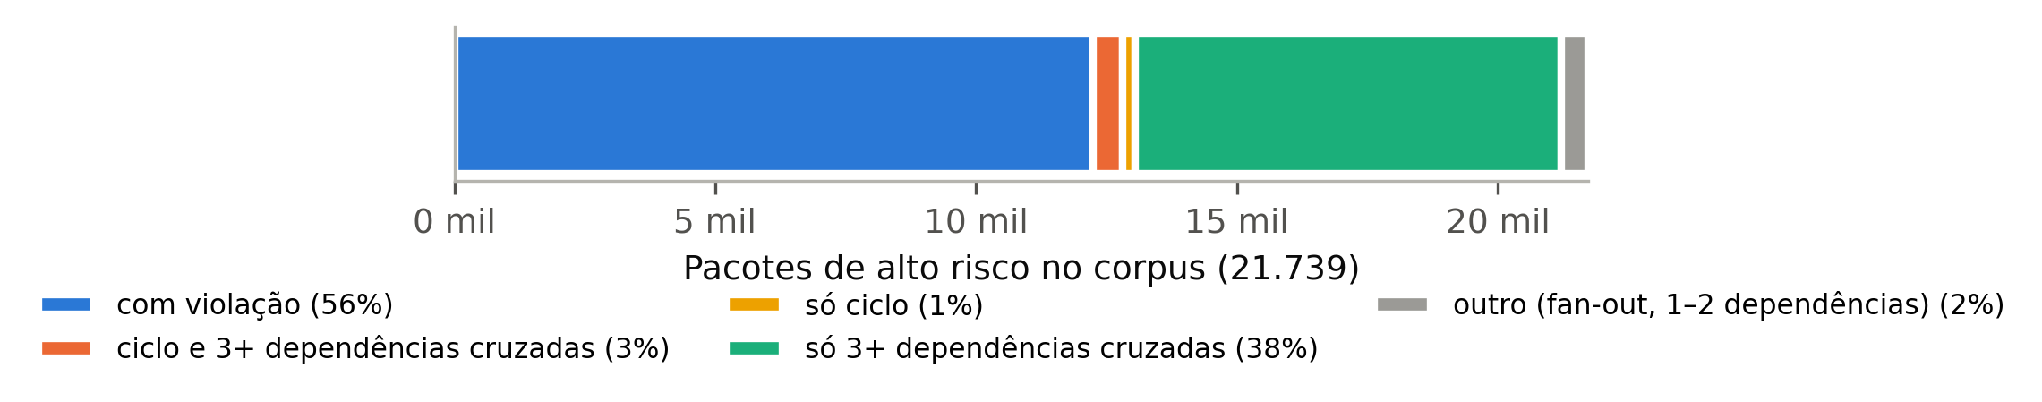
\includegraphics[width=\linewidth,height=0.82\textheight,keepaspectratio]{figures/image2.png}
\caption{Pacotes de alto risco do corpus, separados entre os que têm violação e o motivo estrutural dos que não têm.}
\end{figure}


\hypertarget{qualidade-e-custo-do-nsga-ii}{%
\subsection{Qualidade e custo do NSGA-II}\label{qualidade-e-custo-do-nsga-ii}}

Dos 147 projetos de teste, 143 tinham pacotes candidatos (mediana de 8, máximo de 493). Nos 91 projetos com até 16 candidatos, o NSGA-II alcançou em média 99,9\% do hipervolume da frente exata. Ele encontrou, em média, 86\% dos planos dessa frente, e a frente completa em 70\% dos projetos: os planos que faltam ficam muito próximos dos encontrados e quase não alteram a área coberta. Nos 52 projetos maiores, o NSGA-II e o método guloso praticamente empataram (razão mediana dos hipervolumes de 1,003; NSGA-II maior ou igual em 54\% dos casos), e o desvio-padrão do hipervolume entre cinco sementes foi de 0,0001 na mediana. O empate é esperado: como benefício e esforço somam pacote a pacote, o problema equivale a uma mochila com dois objetivos, para a qual a ordem gulosa é uma boa aproximação. A vantagem do NSGA-II está em entregar a frente inteira de uma vez e em admitir, no futuro, objetivos não aditivos, como o efeito de refatorar um pacote sobre os que dependem dele.

No projeto piloto (Figura 7), com 9 pacotes e 5 candidatos, a frente encontrada coincide com a exata (16 planos), e o plano recomendado indica dois pacotes que, com 29\% do esforço, resolvem 47\% do benefício e 65\% da severidade das violações. Na mediana dos projetos de teste, o plano recomendado toca 22\% dos pacotes e 26\% das linhas de código e obtém 65\% do benefício. \hl{A formulação anterior, de cinco objetivos com fatores simulados, gerava frentes com mediana de 46 planos e um joelho que recomendava refatorar 85\% dos pacotes, o que pouco ajuda a decidir.}

\begin{figure}[htbp]
\centering
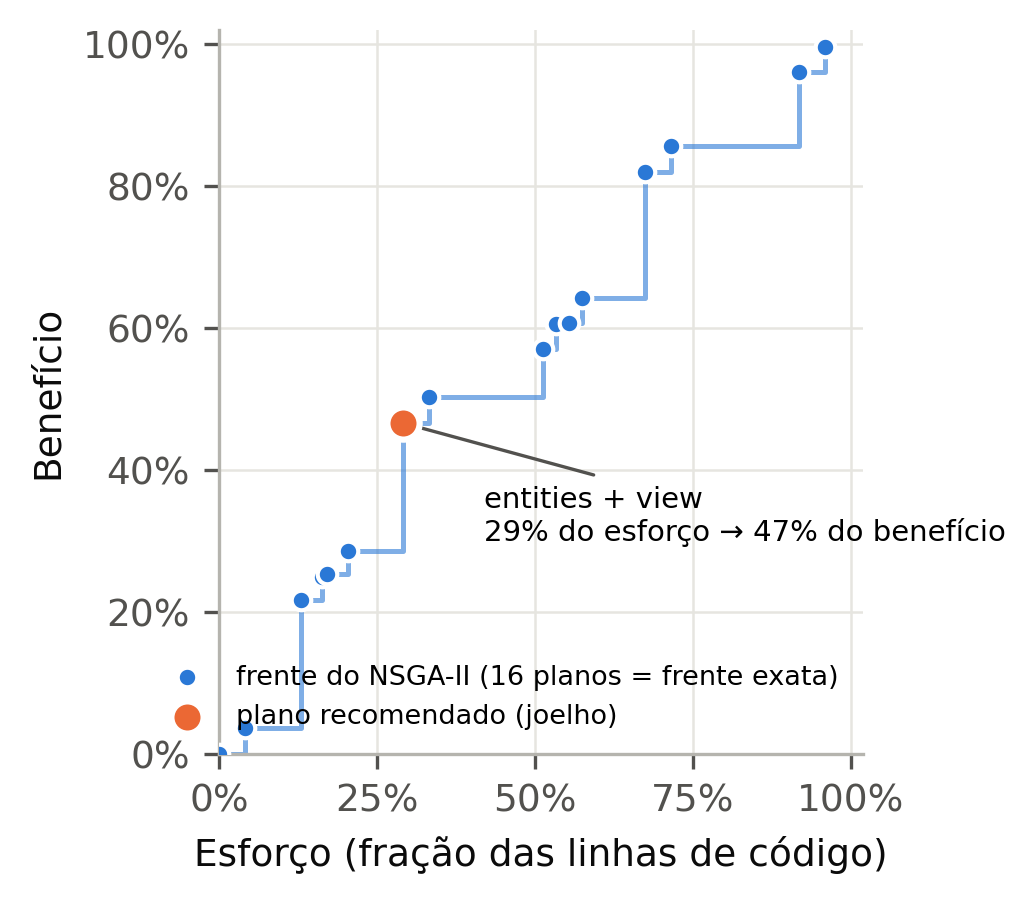
\includegraphics[width=\linewidth,height=0.82\textheight,keepaspectratio]{figures/image7.png}
\caption{Frente de Pareto do NSGA-II no projeto piloto, com o plano recomendado (joelho).}
\end{figure}

\hl{Arrumar o gráfico está com informações sobrepondo o gráfico principal}

O tempo da otimização, incluindo a leitura do grafo, teve mediana de 0,6 s e máximo de 22,5 s, com até 493 candidatos (Figura 8). O tempo cresce com o número de candidatos até cerca de 50 e depois se estabiliza perto de 10 s, porque a população e o número de gerações atingem os tetos de 200 e 300; os maiores tempos vêm, em boa parte, da leitura dos grafos maiores. \hl{A formulação anterior, ao contrário, recortava o subgrafo de cada pacote varrendo o grafo inteiro e ultrapassou 120 s em 2 projetos grandes.} Os resultados estão alinhados com Wolschick et al. (2024), que encontraram o NSGA-II tão bom ou melhor que o NSGA-III em problemas de até três objetivos.

\begin{figure}[htbp]
\centering
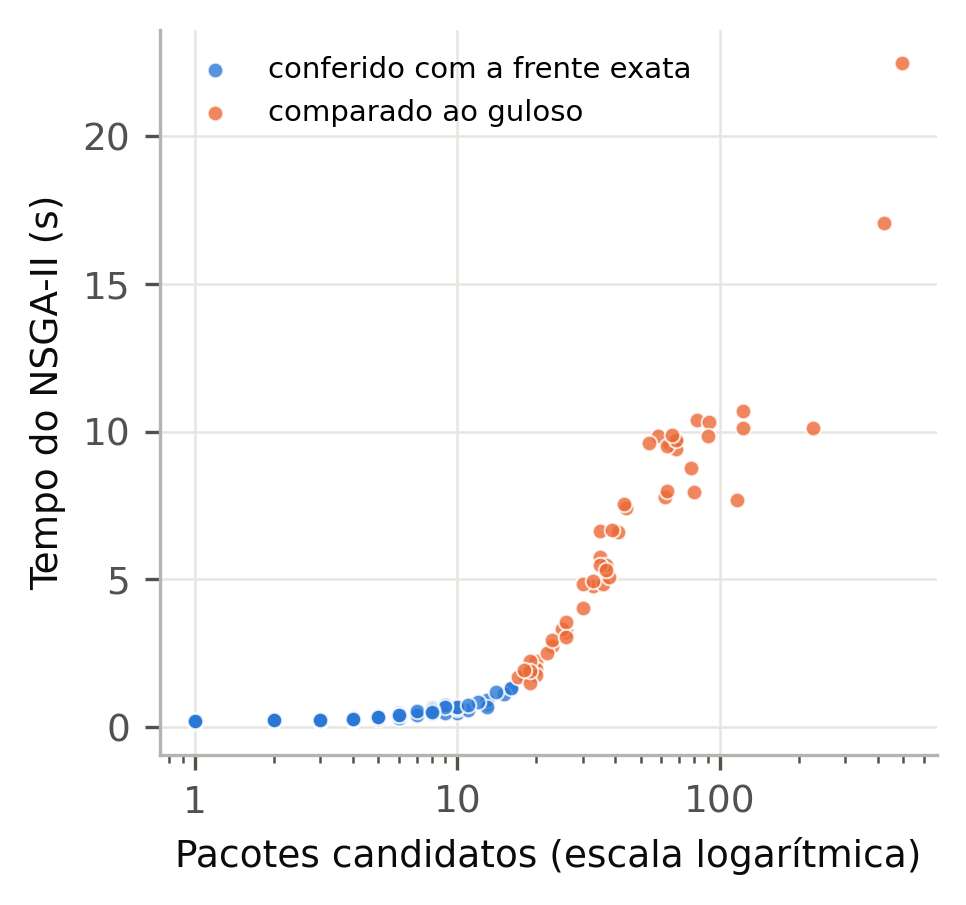
\includegraphics[width=\linewidth,height=0.82\textheight,keepaspectratio]{figures/image6.png}
\caption{Tempo do NSGA-II por projeto de teste em função do número de pacotes candidatos.}
\end{figure}

\hl{Arrumar o gráfico, pois também está sobrepondo informações, revêm de ler e interpretar}

\hypertarget{limites-e-ameauxe7as-uxe0-validade}{%
\subsection{Limites e ameaças à validade}\label{limites-e-ameauxe7as-uxe0-validade}}

\emph{Validade de construto.} O rótulo é um índice derivado das métricas, não uma medida direta de custo de manutenção, e é dominado pelas dependências cruzadas; por isso o modelo foi avaliado também pela localização das violações. \hl{As regras SG\_06 e SG\_11 geram falsos positivos (19,0\% das ocorrências) e, se corrigidas, retirariam 1.331 pacotes (6,1\%) da classe de alto risco; três regras MVC são heurísticas.} Os cortes do índice são calculados no corpus inteiro, e há projetos quase duplicados, embora sua exclusão não tenha alterado os resultados. O corpus contém apenas projetos Java Spring de código aberto do GitHub, com as limitações conhecidas desse tipo de amostra (Kalliamvakou et al., 2014). As métricas do modelo vêm de uma única divisão, mitigada pelos intervalos de confiança por reamostragem de projetos.

\hypertarget{conclusuxe3o}{%
\section{Conclusão}\label{conclusuxe3o}}

Este trabalho apresentou uma abordagem automatizada para priorizar a manutenção arquitetural de sistemas Java Spring e a avaliou em 978 projetos. As violações arquiteturais se concentram em poucos pacotes: os 20\% mais graves reúnem, na mediana, 91,7\% da severidade, acima do que o tamanho dos pacotes explica. O modelo de risco atinge PR-AUC de 98,1\%, mas esse desempenho reflete a reconstrução de um índice estrutural; para localizar violações, ele supera amplamente o acaso e equivale a ordenar os pacotes por tamanho. O NSGA-II alcança 99,9\% do hipervolume da frente exata quando ela pode ser enumerada, empata com um método guloso nos projetos grandes, é estável entre sementes e produz planos interpretáveis em segundos.

As contribuições são o pipeline reprodutível, a evidência em larga escala da concentração de violações arquiteturais, a formulação custo versus benefício verificada do NSGA-II e o alerta metodológico de que a acurácia contra um rótulo derivado das próprias entradas não mede a utilidade de um modelo de risco. As principais limitações são o rótulo estrutural, \hl{o excesso de alcance de duas regras Singleton} e a restrição a projetos de código aberto.

Como trabalhos futuros, propõem-se: treinar o modelo com um rótulo baseado apenas nas violações e compará-lo com o tamanho; \hl{corrigir as regras SG\_06 e SG\_11}; dividir o corpus por dono do repositório; avaliar a ferramenta em projetos fora do corpus e em sistemas de empresas; e incorporar a preferência do arquiteto durante a busca, como no operador interativo de Rosa et al.~(2022).

\hypertarget{referuxeancias}{%
\section{Referências}\label{referuxeancias}}

Assunção, W. K. G., Colanzi, T. E., Vergilio, S. R., \& Pozo, A. T. R. (2013). Generating integration test orders for aspect-oriented software with multi-objective algorithms. \emph{Revista de Informática Teórica e Aplicada, 20}(2), 301-327.

Basili, V. R., Briand, L. C., \& Melo, W. L. (1996). A validation of object-oriented design metrics as quality indicators. \emph{IEEE Transactions on Software Engineering, 22}(10), 751-761. https://doi.org/10.1109/32.544352

Boehm, B., \& Basili, V. R. (2001). Software defect reduction top 10 list. \emph{Computer, 34}(1), 135-137. https://doi.org/10.1109/2.962984

Borowski, K., Baliś, B., \& Orzechowski, T. (2024). Semantic Code Graph: an information model to facilitate software comprehension. \emph{IEEE Access, 12}, 27279-27310. https://doi.org/10.1109/ACCESS.2024.3366822

Colanzi, T. E., \& Vergilio, S. R. (2016). A feature-driven crossover operator for multi-objective and evolutionary optimization of product line architectures. \emph{Journal of Systems and Software}. https://doi.org/10.1016/j.jss.2016.02.026

Crotty, J., \& Horrocks, I. (2017). \emph{Managing legacy system costs: a case study of a meta-assessment model to identify solutions in a large financial services company}. The Open University.

de Silva, L., \& Balasubramaniam, D. (2012). Controlling software architecture erosion: a survey. \emph{Journal of Systems and Software, 85}(1), 132-151. https://doi.org/10.1016/j.jss.2011.07.036

Deb, K., Pratap, A., Agarwal, S., \& Meyarivan, T. (2002). A fast and elitist multiobjective genetic algorithm: NSGA-II. \emph{IEEE Transactions on Evolutionary Computation, 6}(2), 182-197. https://doi.org/10.1109/4235.996017

Duvvur, V. (2023). Cost-benefit analysis of legacy system modernization: a critical evaluation for informed decision-making. \emph{ESP Journal of Engineering \& Technology Advancements, 3}(3), 37-40. https://doi.org/10.56472/25832646/JETA-V3I7P106

Efron, B., \& Tibshirani, R. J. (1993). \emph{An introduction to the bootstrap}. Chapman \& Hall.

Fenton, N. E., \& Ohlsson, N. (2000). Quantitative analysis of faults and failures in a complex software system. \emph{IEEE Transactions on Software Engineering, 26}(8), 797-814. https://doi.org/10.1109/32.879815

Harman, M. (2007). The current state and future of search based software engineering. In \emph{Future of Software Engineering (FOSE \textquotesingle07)} (pp. 342-357). IEEE. https://doi.org/10.1109/FOSE.2007.29

Harman, M., \& Jones, B. F. (2001). Search-based software engineering. \emph{Information and Software Technology, 43}(14), 833-839. https://doi.org/10.1016/S0950-5849(01)00189-6

Hu, R. (2023). \emph{An automated approach to check software architecture erosion} {[}Dissertação de mestrado{]}. Eindhoven University of Technology.

Irani, Z., Abril, R. M., Weerakkody, V., Omar, A., \& Sivarajah, U. (2023). The impact of legacy systems on digital transformation in European public administration: lesson learned from a multi case analysis. \emph{Government Information Quarterly}.

Kalliamvakou, E., Gousios, G., Blincoe, K., Singer, L., German, D. M., \& Damian, D. (2014). The promises and perils of mining GitHub. In \emph{Proceedings of the 11th Working Conference on Mining Software Repositories} (pp.~92-101). ACM. https://doi.org/10.1145/2597073.2597074

Li, R., Liang, P., Soliman, M., \& Avgeriou, P. (2022). Understanding software architecture erosion: a systematic mapping study. \emph{Journal of Software: Evolution and Process, 34}(3), e2423. https://doi.org/10.1002/smr.2423

Liu, J., et al.~(2024). 3Erefactor: effective, efficient and executable refactoring recommendation for software architectural consistency. \emph{IEEE Transactions on Software Engineering, 50}(10), 2633-2654. https://doi.org/10.1109/TSE.2024.3449564

Martin, R. C. (2003). \emph{Agile software development: principles, patterns, and practices}. Prentice Hall.

Melton, H., \& Tempero, E. (2007). An empirical study of cycles among classes in Java. \emph{Empirical Software Engineering, 12}(4), 389-415.

Mende, T., \& Koschke, R. (2010). Effort-aware defect prediction models. In \emph{14th European Conference on Software Maintenance and Reengineering} (pp.~107-116). IEEE. https://doi.org/10.1109/CSMR.2010.18

Ostrand, T. J., Weyuker, E. J., \& Bell, R. M. (2005). Predicting the location and number of faults in large software systems. \emph{IEEE Transactions on Software Engineering, 31}(4), 340-355. https://doi.org/10.1109/TSE.2005.49

Oyetoyan, T. D., Cruzes, D. S., \& Conradi, R. (2013). A study of cyclic dependencies on defect profile of software components. \emph{Journal of Systems and Software, 86}(12), 3162-3182.

Perry, D. E., \& Wolf, A. L. (1992). Foundations for the study of software architecture. \emph{ACM SIGSOFT Software Engineering Notes, 17}(4), 40-52. https://doi.org/10.1145/141874.141884

Rosa, C. T., Freire, W. M., Amaral, A. M. M. M., \& Colanzi, T. E. (2022). Towards an interactive ranking operator for NSGA-II. In \emph{Genetic and Evolutionary Computation Conference Companion (GECCO \textquotesingle22 Companion)}. ACM. https://doi.org/10.1145/3520304.3529041

Saito, T., \& Rehmsmeier, M. (2015). The precision-recall plot is more informative than the ROC plot when evaluating binary classifiers on imbalanced datasets. \emph{PLOS ONE, 10}(3), e0118432. https://doi.org/10.1371/journal.pone.0118432

Satopää, V., Albrecht, J., Irwin, D., \& Raghavan, B. (2011). Finding a "kneedle" in a haystack: detecting knee points in system behavior. In \emph{31st International Conference on Distributed Computing Systems Workshops} (pp.~166-171). IEEE. https://doi.org/10.1109/ICDCSW.2011.20

Venâncio, A. L. A. C., Brezinski, G. L., Leal, G. S. S., Loures, E. F. R., \& Deschamps, F. (2022). Digital transformation in maintenance: interoperability-based adequacy aiming smart legacy systems.

Wilcoxon, F. (1945). Individual comparisons by ranking methods. \emph{Biometrics Bulletin, 1}(6), 80-83. https://doi.org/10.2307/3001968

Wolschick, L., Gonçalves, P. C., Choma Neto, J., Freire, W. M., Amaral, A. M. M. M., \& Colanzi, T. E. (2024). Evaluating the performance of NSGA-II and NSGA-III on product line architecture design. In \emph{Anais do XVIII Simpósio Brasileiro de Componentes, Arquiteturas e Reutilização de Software (SBCARS 2024)}. SBC.

Zimmermann, T., \& Nagappan, N. (2008). Predicting defects using network analysis on dependency graphs. In \emph{Proceedings of the 30th International Conference on Software Engineering} (pp.~531-540). ACM. https://doi.org/10.1145/1368088.1368161

Zitzler, E., \& Thiele, L. (1999). Multiobjective evolutionary algorithms: a comparative case study and the strength Pareto approach. \emph{IEEE Transactions on Evolutionary Computation, 3}(4), 257-271. \href{https://doi.org/10.1109/4235.797969}{\ul{https://doi.org/10.1109/4235.797969}}

\end{document}
